\chapter{ReSPect: Residual Spectral Prediction}\label{ch:respect}

This chapter presents ReSPect (Residual Spectral Prediction for Efficient Caching of Transformers), the first method developed in this project. ReSPect is a training-free cache for diffusion transformers that combines the spectrally aligned gate of \cref{sec:bg-sea} with a forecaster of the skipped \emph{residuals}. The forecaster is a weighted sum of a ridge-regularised Chebyshev regression over the accumulated residual history, which captures the global trajectory, and a first-order discrete Taylor correction, which captures local dynamics. We show that its forecast error admits a skip-length-independent bound, whereas the bounds of copy-reuse and Taylor extrapolation grow with the skip length, and we derive its blend weight and warm-up length analytically. On FLUX.1-dev, Wan2.1-1.3B and HunyuanVideo, ReSPect achieves speedups of $3.30\times$, $2.63\times$ and $2.77\times$ over full evaluation with lower output error than existing caching baselines at matched or lower compute. The chapter follows our ReSPect paper, with the derivations given in full and an additional description of the implementation.

\begin{figure}[t]
  \centering
  
\includegraphics[width=0.95\textwidth]{respect_teaser.pdf}
  \caption[Images generated with ReSPect on FLUX.1-dev]{Images generated by FLUX.1-dev with ReSPect, which keeps high image fidelity at a $2.43\times$ acceleration.}
  \label{fig:respect-teaser}
\end{figure}

%% ------------------------------------------------------------------------------------------------
\section{Motivation}\label{sec:respect-motivation}

As discussed in \cref{sec:lit-accel}, a cache makes two coupled decisions at every step: a schedule decides whether the network is evaluated, and a reconstructor decides what is written to the features when it is not. Improving either one in isolation leaves the other as the bottleneck. The literature review identified two limitations:
\begin{itemize}
  \item \textbf{Noisy schedules.} Many gates use the raw distance between consecutive features \citep{liu2025teacache,bu2025dicache}. Under the mixture $x_t=a_tx_0+b_t\epsilon$ the noise contribution can dominate this distance at early steps, so the gate responds to stochastic variation. A timestep-dependent spectral filter isolates the content-sensitive drift (\cref{sec:bg-sea}).
  \item \textbf{Local reconstructors.} Most reconstructors use local temporal information, copying the last computed features \citep{selvaraju2024fora,zhao2024pab} or extrapolating from finite differences \citep{liu2025taylorseer}. Their approximation error grows with the skip length, and sample quality degrades at high speedups. Global trajectory fitting \citep{han2026spectrum} still predicts the full hidden state.
\end{itemize}
ReSPect specifies both decisions together (\cref{fig:respect-overview}). It keeps the spectrally aligned gate and forecasts only the transformer residual, because the block input at skipped steps is known exactly. This removes the predictable component from the regression target and yields a smaller, centred trajectory.

\begin{figure}[t]
  \centering
  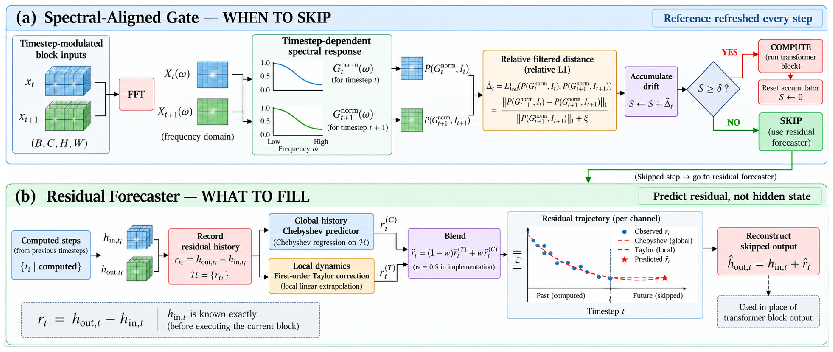
\includegraphics[width=\textwidth]{respect_overview.pdf}
  \caption[Overview of ReSPect]{Overview of ReSPect. (a) The spectrally aligned gate decides adaptively when to evaluate the network. (b) The residual forecaster combines a global Chebyshev prediction with a local first-order Taylor correction and writes $h^{\mathrm{in}}+\hat r$ on skipped steps.}
  \label{fig:respect-overview}
\end{figure}

%% ------------------------------------------------------------------------------------------------
\section{Problem setup}\label{sec:respect-setup}

Consider a latent generative model whose sampling trajectory $\{x_t\}_{t=0}^T$ is produced by a discrete solver, where $t\in\{0,\dots,T\}$ indexes solver steps from the initial noise towards the clean output. At step $t$ the latent $x_t$ is mapped to the input $I_t=\phi(x_t,t)$ of a transformer block, whose output $h^{\mathrm{out}}(t)$ is produced from the input $h^{\mathrm{in}}(t)$. The block residual
\begin{equation}\label{eq:respect-residual}
  r(t) = h^{\mathrm{out}}(t) - h^{\mathrm{in}}(t)
\end{equation}
induces a second trajectory $\{r(t)\}$ alongside $\{x_t\}$. On an evaluated step $h^{\mathrm{out}}(t)=h^{\mathrm{in}}(t)+r(t)$ holds by definition. On a skipped step the input is known and the reconstructor supplies $\hat r(t)$, yielding $\hat h^{\mathrm{out}}(t) = h^{\mathrm{in}}(t)+\hat r(t)$, so that the reconstruction error coincides with the residual error,
\begin{equation}\label{eq:respect-errid}
  \hat h^{\mathrm{out}}(t) - h^{\mathrm{out}}(t) = \hat r(t) - r(t)
\end{equation}
(\cref{eq:bg-error}). The reconstruction problem is therefore reduced to forecasting the residual trajectory at unevaluated steps.

\paragraph{The gate.} ReSPect uses the spectrally aligned gate of \cref{sec:bg-sea} unchanged in form: the first-block input is filtered with the gain-normalised Wiener response $G^{\mathrm{norm}}_t$ of \cref{eq:bg-wiener,eq:bg-norm}, each adjacent pair $(I_t,I_{t+1})$ is compared with its own pair of responses,
\begin{equation}
  \tilde\Delta_t = \Lone\big(\mathcal P(G^{\mathrm{norm}}_t,I_t),\,\mathcal P(G^{\mathrm{norm}}_{t+1},I_{t+1})\big), \qquad \mathcal P(G,I) = \mathcal F^{-1}\big[G\odot\mathcal F(I)\big],
\end{equation}
and the network is evaluated when the accumulated $\tilde\Delta_t$ exceeds $\delta$. The reference is refreshed at every step, including skipped steps, so each $\tilde\Delta_t$ measures only the incremental drift; on HunyuanVideo this choice is worth $+2.50$\,dB at matched compute (\cref{sec:respect-ablations}). The rest of this chapter specifies what is written on the skipped steps.

%% ------------------------------------------------------------------------------------------------
\section{Predictors on the sampling trajectory}\label{sec:respect-hierarchy}

We state the analysis for one residual channel; the predictor is applied independently across channels. Consider a skip from the last evaluated step $t_k$ to the current step $t_j$. Every reconstructor is a predictor $\hat r(t_j)$ built from the residuals recorded at evaluated steps; the candidates differ in the smoothness they assume of $r$.

\subsection{Order zero: copy-reuse}
Copy-reuse sets $\hat r(t_j)=r(t_k)$. If $r$ is $L$-Lipschitz on the sampling interval, then directly from the definition
\begin{equation}\label{eq:respect-reuse}
  |r(t_j)-r(t_k)| \le L\,|t_j-t_k| .
\end{equation}
The bound is tight, since $r(t)=Lt$ attains equality for every skip, and Lipschitz continuity is necessary in the worst case: for a non-Lipschitz residual the ratio $|r(t_j)-r(t_k)|/|t_j-t_k|$ is unbounded as the skip shrinks. Copy-reuse uses no derivative information, so additional smoothness ($r\in C^P$, $P\ge 1$) cannot improve the worst-case rate. \emph{The error of reuse grows linearly with the skip length.}

\subsection{Order $P$: Taylor extrapolation}
Assume $r\in C^{P+1}$. The degree-$P$ Taylor expansion of $r$ about $t_k$ is
\begin{equation}
  r(t_j) = \sum_{p=0}^{P}\frac{r^{(p)}(t_k)}{p!}(t_j-t_k)^p + R_P(t_j), \qquad R_P(t_j) = \frac{r^{(P+1)}(\xi)}{(P+1)!}(t_j-t_k)^{P+1}
\end{equation}
for some $\xi$ between $t_k$ and $t_j$. Hence $|R_P(t_j)|\le \|r^{(P+1)}\|_\infty |t_j-t_k|^{P+1}/(P+1)!$, an order-$(P{+}1)$ dependence on the skip length \citep[Thm.~3.1]{han2026spectrum}. This is the \emph{ideal} predictor, because it uses the exact derivatives at $t_k$, which a training-free cache never computes.

\paragraph{The implemented (discrete) predictor.} In practice the derivatives are replaced by backward differences formed from $P{+}1$ neighbouring evaluated residuals $s_0=t_k,s_1,\dots,s_P$, so the predictor is the degree-$P$ interpolant $p_P$ through those nodes, with remainder
\begin{equation}\label{eq:respect-interp}
  r(t_j)-p_P(t_j) = \frac{r^{(P+1)}(\xi)}{(P+1)!}\prod_{q=0}^{P}(t_j-s_q)
\end{equation}
for some $\xi$ in the convex hull of $\{t_j,s_0,\dots,s_P\}$. Only the $q=0$ factor shrinks with the skip length $\ell=|t_j-t_k|$; the remaining factors are fixed by the positions of the earlier evaluated nodes. The $(P{+}1)$-order rate therefore requires a node-spacing condition $\max_q|t_j-s_q|\le C_{\mathrm{node}}\,\ell$, under which $|r(t_j)-p_P(t_j)|\le C_{\mathrm{node}}^{P+1}\|r^{(P+1)}\|_\infty\,\ell^{P+1}/(P+1)!$. A dynamic gate does not guarantee a uniform $C_{\mathrm{node}}$: with the earlier nodes held fixed and $\ell\to 0$, the error is $O(\ell)$, not $O(\ell^{P+1})$.

\begin{proposition}[The failure is sharp]\label{prop:respect-sharp}
Take $P=1$, $r(t)=t^2$, nodes $s_0=t_k=0$ and $s_1=-H$ with $H>0$, and forecast point $t_j=\ell>0$. Then $|r(\ell)-p_1(\ell)|/\ell^2 = 1 + H/\ell$, which is unbounded as $H/\ell\to\infty$.
\end{proposition}
\begin{proof}
The linear interpolant through $(0,0)$ and $(-H,H^2)$ is $p_1(t)=-Ht$, so $|r(\ell)-p_1(\ell)| = \ell^2+H\ell = \ell(\ell+H)$. Dividing by $\ell^2$ gives the claim.
\end{proof}

Even uniform backward spacing does not recover the ideal rate: for $t_j=t_k+\ell$ and $s_q=t_k-qh$, $\prod_{q=0}^P|t_j-s_q|=\prod_{q=0}^P(\ell+qh)$ is a degree-$(P{+}1)$ polynomial in $\ell$ that coincides with $\ell^{P+1}$ only in the limit $h/\ell\to 0$. In addition, the difference operator amplifies observation noise by binomial coefficients of order $2^P$. A higher order therefore tightens the bound only for short skips and becomes unstable as $|t_j-t_k|$ grows, and the predictor discards all but the $P{+}1$ most recent evaluations. These bounds motivate a \emph{global} predictor that exploits the full observed trajectory.

%% ------------------------------------------------------------------------------------------------
\section{Residual forecasting with Chebyshev bases}\label{sec:respect-cheb}

To predict $r(t_j)$ we fit the accumulated residual trajectory. The solver-step index is mapped affinely from the fixed solver-step range to $\tau\in[-1,1]$, and each residual channel (of feature dimension $F$) is expanded in the Chebyshev basis $T_0,\dots,T_M$ of degree $M$ (\cref{fig:lit-chebyshev}). Stack the $K$ recorded residuals row-wise into the observation matrix $H\in\R^{K\times F}$, let $\Phi\in\R^{K\times(M+1)}$ evaluate the basis at the recorded steps, and regress the coefficient matrix $C\in\R^{(M+1)\times F}$ with ridge penalty $\lambda$ \citep{hoerl1970ridge}:
\begin{equation}\label{eq:respect-ridge}
  C^\star = \arg\min_C \|\Phi C - H\|_F^2 + \lambda\|C\|_F^2 = (\Phi\tr\Phi+\lambda I)^{-1}\Phi\tr H .
\end{equation}
The fit is re-solved whenever a new residual is computed; the window retains the last $K$ observations, which exceeds the number of solver steps in all reported runs. The forecast at a skipped step evaluates the fitted expansion at its coordinate, $\hat r(t_j)=\sum_{m=0}^M \hat C_m T_m(\tau_j)$.

\paragraph{Truncation error.} Let $p^\star_M$ be the exact degree-$M$ Chebyshev truncation of $r$. Assume that $r$ extends analytically to the Bernstein ellipse $E_\rho$ ($\rho>1$, foci $\pm1$, semi-axis sum $\rho$) on which $|r|\le B$. The Chebyshev coefficients have the contour representation $c_m = \frac{1}{\pi i}\oint_{E_\rho} r(z)\,T_m(z)^{-1}\,dz/z$ (up to the standard factor for $m=0$), and on $E_\rho$ one has $|T_m|\ge(\rho^m-\rho^{-m})/2$, which yields $|c_m|\le 2B\rho^{-m}$ for $m\ge1$ and $|c_0|\le B$. Since $|T_m(\tau)|\le 1$ on $[-1,1]$, truncating at degree $M$ leaves \citep[Thm.~3.2]{han2026spectrum}
\begin{equation}\label{eq:respect-trunc}
  \|r-p^\star_M\|_\infty \le \sum_{m=M+1}^{\infty}2B\rho^{-m} = \frac{2B}{\rho-1}\rho^{-M}.
\end{equation}
The right-hand side depends on $M$, $\rho$ and $B$, but not on the evaluation point: \emph{the approximation-theoretic term is independent of the skip length}. Because the coefficients are estimated from finitely many observations, we also control the deviation of the estimator from the ideal truncation.

\begin{lemma}[Ridge stability; restated from {\citealp[Thm.~3.3]{han2026spectrum}}]\label{lem:respect-ridge}
Let $\hat r$ be the Chebyshev component from \cref{eq:respect-ridge}, $p^\star_M$ the exact degree-$M$ truncation and $\sigma_{\min}=\sigma_{\min}(\Phi)$ (zero whenever $K<M+1$). At any forecast coordinate $\tau_j$,
\begin{equation}\label{eq:respect-lemma}
  |\hat r(\tau_j)-p^\star_M(\tau_j)| \le \varepsilon_M\,\frac{(M+1)K}{\sigma_{\min}^2+\lambda} + \frac{\lambda\sqrt{M+1}}{\sigma_{\min}^2+\lambda}\cdot\frac{2B}{\sqrt{1-\rho^{-2}}},
\end{equation}
where $\varepsilon_M$ is the right-hand side of \cref{eq:respect-trunc}.
\end{lemma}
\begin{proof}
Fix one channel and take $\lambda>0$. Write the $K$ observations as $y=\Phi c^\star+e$, where $c^\star$ are the exact Chebyshev coefficients of $p^\star_M$ and, by \cref{eq:respect-trunc}, $|e_k|\le\varepsilon_M$, so $\|e\|_2\le\sqrt K\varepsilon_M$. The ridge estimate is $\hat c=(\Phi\tr\Phi+\lambda I)^{-1}\Phi\tr y$, hence
\begin{equation}
  \hat c - c^\star = (\Phi\tr\Phi+\lambda I)^{-1}\Phi\tr e - \lambda(\Phi\tr\Phi+\lambda I)^{-1}c^\star .
\end{equation}
The forecast error is the inner product of $\hat c-c^\star$ with the basis row $\varphi(\tau_j)=[T_0(\tau_j),\dots,T_M(\tau_j)]$, and $\|\varphi(\tau_j)\|_2\le\sqrt{M+1}$.

\emph{Variance term.} With the singular values $\sigma_1\ge\dots\ge\sigma_{M+1}=\sigma_{\min}$ of $\Phi$,
$\|(\Phi\tr\Phi+\lambda I)^{-1}\Phi\tr\|_2 = \max_i \sigma_i/(\sigma_i^2+\lambda) \le \sigma_1/(\sigma_{\min}^2+\lambda)$, and since every entry of $\Phi$ is bounded by one, $\sigma_1\le\|\Phi\|_F\le\sqrt{(M+1)K}$. Therefore
\begin{equation}
  \big|\varphi(\tau_j)(\Phi\tr\Phi+\lambda I)^{-1}\Phi\tr e\big| \le \sqrt{M+1}\cdot\frac{\sqrt{(M+1)K}}{\sigma_{\min}^2+\lambda}\cdot\sqrt K\varepsilon_M = \frac{(M+1)K}{\sigma_{\min}^2+\lambda}\,\varepsilon_M .
\end{equation}

\emph{Bias term.} The coefficient bound $|c^\star_m|\le 2B\rho^{-m}$ gives $\|c^\star\|_2\le 2B\big(\sum_{m\ge0}\rho^{-2m}\big)^{1/2} = 2B/\sqrt{1-\rho^{-2}}$, independent of $M$. The eigenvalues of $(\Phi\tr\Phi+\lambda I)^{-1}$ are $1/(\sigma_i^2+\lambda)$, so its spectral norm is $1/(\sigma_{\min}^2+\lambda)$ and
\begin{equation}
  \big|\varphi(\tau_j)\,\lambda(\Phi\tr\Phi+\lambda I)^{-1}c^\star\big| \le \frac{\lambda\sqrt{M+1}}{\sigma_{\min}^2+\lambda}\cdot\frac{2B}{\sqrt{1-\rho^{-2}}} .
\end{equation}
Adding the two bounds proves the lemma.
\end{proof}

Adding $\varepsilon_M$ once more by the triangle inequality bounds the total error $|r(\tau_j)-\hat r(\tau_j)|$. The two terms expose a trade-off. Each observation adds a positive semi-definite rank-one term to $\Phi\tr\Phi$, so $\sigma_{\min}$ is non-decreasing in $K$ and the factor $K/(\sigma_{\min}^2+\lambda)$ stays bounded rather than growing; before $K$ reaches $M{+}1$ the design is rank-deficient and $\lambda$ alone controls the bound, at the price of bias. \Cref{sec:respect-blend} turns this condition into an explicit warm-up threshold.

\paragraph{Node spacing versus design conditioning.} The node-spacing condition of the Taylor analysis and the design conditioning $\sigma_{\min}(\Phi)$ of \cref{lem:respect-ridge} are distinct properties of the realised schedule, and neither implies the other. If the forecast distance $\ell$ stays fixed while the earlier nodes coalesce onto $t_k$, the spacing condition holds with $C_{\mathrm{node}}\to1$, yet the rows of $\Phi$ become nearly identical and $\sigma_{\min}\to0$. Conversely, a fixed well-spread design keeps $\sigma_{\min}$ bounded away from zero, while a forecast with $\ell\to0^+$ against a fixed distant node drives $\max_q|t_j-s_q|/\ell\to\infty$. Each analysis therefore controls a separate failure mode.

%% ------------------------------------------------------------------------------------------------
\section{Why forecast the residual?}\label{sec:respect-residual-space}

On a skipped step the block input $h^{\mathrm{in}}$ is known exactly from the current sampling state. For a state forecast $\hat h^{\mathrm{out}}$ and a residual forecast $\hat r$,
\begin{equation}
  \hat h^{\mathrm{out}} - h^{\mathrm{out}} = (\hat r + h^{\mathrm{in}}) - (r + h^{\mathrm{in}}) = \hat r - r .
\end{equation}
Once the predictor is fixed, state and residual formulations therefore have identical reconstruction error; they differ only in their regression target. Stacking the observed rows gives the exact identity $H_{\mathrm{out}} = H_{\mathrm{in}} + R$, where $H_{\mathrm{in}}$ varies with the step and is not rank one, so no low-rank structure is assumed. Each hidden-state observation carries the large input component, which the sampler already knows; fitting the full state inflates the regression target without adding anything that needs predicting. The ridge map is linear in its target, so scaling the target scales the fitted coefficients and the absolute shrinkage bias, while the shrinkage factor $\lambda/(\sigma_{\min}^2+\lambda)$ is unchanged. The constants of \cref{lem:respect-ridge} scale with the target norm through $B$. Forecasting $R$ directly keeps the target small-normed and tightens every constant in proportion. This is a target-scale advantage rather than a conditioning one, since all fits share the same design matrix $\Phi$. The analysis assumes that the residual trajectory satisfies the same analyticity condition with comparable $\rho$; consistently, the $M$-sweep of \cref{tab:respect-msweep} saturates at the same small $M$ used throughout. The skipped-step update is simply $h\leftarrow h+\hat r$.

%% ------------------------------------------------------------------------------------------------
\section{Analytic blend and warm-up}\label{sec:respect-blend}

\paragraph{Blend.} The forecast is a convex combination of the discrete Taylor predictor $\hat r_T$ and the Chebyshev predictor $\hat r_C$,
\begin{equation}
  \hat r_w = (1-w)\,\hat r_T + w\,\hat r_C .
\end{equation}
For the risk model we assign the Taylor predictor's systematic error to a squared bias $b_T^2$ and the Chebyshev estimator's finite-history uncertainty to a variance $\sigma_C^2$, and treat the two errors as uncorrelated. Omitting $w$-independent terms, the risk is
\begin{equation}\label{eq:respect-risk}
  R(w) = (1-w)^2 b_T^2 + w^2\sigma_C^2 ,
\end{equation}
and setting $R'(w)=0$ gives $w^\star = b_T^2/(b_T^2+\sigma_C^2)$. Early in sampling the drift is fast ($b_T$ large) and the fit has seen few points ($\sigma_C$ large); later both decrease as the trajectory settles and observations accumulate. Measured trajectories keep the two terms within a factor of two of each other, which places $w^\star$ near $1/2$ throughout. Because the bias and variance are not observable at inference time, we use the symmetric fixed weight $w=0.5$, which needs no adaptation or hyper-parameter search. \Cref{sec:respect-ablations} shows that this choice is robust across models and budgets, whereas $w=1$ removes the low-bias local term precisely when the polynomial fit is least determined.

\paragraph{Warm-up.} With $n<M+1$ observations, \cref{eq:respect-ridge} is rank-deficient ($\sigma_{\min}=0$), the observations cannot identify all coefficient directions, and the fit is dominated by the penalty (the bias term of \cref{lem:respect-ridge}). The first-order discrete Taylor step is exact on the last two observations by construction and therefore strictly dominates in this regime: it reduces to copy-reuse at $n=1$ and extrapolates linearly from $n=2$ onward. In practice the regularised fit is determined one observation early, so blending starts at $n\ge4$ (with $M=4$) rather than at $M+1$. The warm-up is thus the degrees-of-freedom crossover rather than a tuned choice.

\paragraph{Compute and memory.} Skip decisions accumulate per sample, so prompts in a batch never share a schedule. Each sample stores one $(M{+}1)\times F$ coefficient matrix and $K$ recorded residuals, i.e.\ $O((M+1)F+KF)$ memory, with fitting cost $O(K(M+1)F)$ for $M\ll K\ll F$ (the $(M+1)^3$ Cholesky term is negligible) and prediction cost $O((M+1)F)$. The measured overhead is about 0.09\,s per FLUX.1-dev image.

\Cref{alg:respect} summarises the complete procedure.

\begin{algorithm}[t]
\caption{ReSPect sampling (one sample)}\label{alg:respect}
\begin{algorithmic}[1]
\Require initial noise $x_0$, solver with $N$ steps, threshold $\delta$; $M{=}4$, $K{=}100$, $\lambda{=}0.1$, $w{=}0.5$
\State $D\gets 0$; history $\mathcal H\gets\emptyset$; $I_{\mathrm{prev}}\gets$ none
\For{$t = 0,\dots,N-1$}
  \State $h^{\mathrm{in}}\gets \Emb(x_t)$; \quad $\tilde I\gets \mathcal P(G^{\mathrm{norm}}_t, \mathrm{AdaLN}_0(h^{\mathrm{in}}, c_t))$
  \If{$t\in\{0,N-1\}$ \textbf{or} $I_{\mathrm{prev}}$ is none}
     \State compute $\gets$ true; $D\gets0$
  \Else
     \State $D\gets D+\Lone(\tilde I, I_{\mathrm{prev}})$; \quad compute $\gets (D\ge\delta)$; \textbf{if} compute \textbf{then} $D\gets 0$
  \EndIf
  \State $I_{\mathrm{prev}}\gets\tilde I$ \Comment{reference refreshed at every step}
  \If{compute}
     \State $r\gets F(h^{\mathrm{in}})-h^{\mathrm{in}}$; append $(t,r)$ to $\mathcal H$ (keep last $K$); refit $C^\star$ by \cref{eq:respect-ridge}
  \Else
     \State $\hat r_T\gets$ first-order discrete Taylor step from the last two entries of $\mathcal H$
     \If{$|\mathcal H|\ge4$} $r\gets(1-w)\hat r_T + w\sum_m C^\star_m T_m(\tau_t)$ \Else\ $r\gets\hat r_T$ \EndIf
  \EndIf
  \State $v_t\gets\Out(h^{\mathrm{in}}+r, c_t)$; \quad $x_{t+1}\gets\mathrm{SolverStep}(x_t, v_t)$
\EndFor
\State \Return $x_N$
\end{algorithmic}
\end{algorithm}

%% ------------------------------------------------------------------------------------------------
\section{Implementation}\label{sec:respect-impl}

The ReSPect code release follows the layout of SeaCache: one self-contained folder per backbone, each with a copy of the SEA filter (\texttt{util\_seacache.py}), the forecaster (\texttt{spectrum\_forecaster.py}) and a generate script (\texttt{respect\_generate.py}). Key excerpts are reproduced in \cref{app:code}.
\begin{itemize}
  \item \textbf{FLUX.1-dev (diffusers).} The script replaces \texttt{FluxTransformer2DModel.forward} at import time. The gate takes the first double-stream block's \texttt{norm1} output, lays it out on its $(H,W)$ token grid using the rotary image ids, applies the SEA filter with $\beta=2$ over the two spatial axes, and accumulates the relative $\ell_1$ distance. A fresh \texttt{SpectrumResidualForecaster} is created for every image, so the forecaster state never leaks between prompts. Command-line flags: \texttt{--seacache\_thresh} ($\delta$) and \texttt{--spectrum\_m/k/lam/w/min\_cheb\_obs}.
  \item \textbf{Wan2.1.} The script is a copy of the official \texttt{generate.py} with patched \texttt{t2v\_generate}, \texttt{i2v\_generate} and model forward. Classifier-free guidance calls the transformer twice per step; the two calls alternate, so the gate and the forecaster keep separate states for the even (conditional) and odd (unconditional) calls, with step index $\lfloor\mathrm{cnt}/2\rfloor$.
  \item \textbf{HunyuanVideo.} The forward of \texttt{HYVideoDiffusionTransformer} is replaced on the loaded sampler. Because HunyuanVideo residuals are large, the ridge solve is chunked over the feature dimension (\texttt{fit\_chunks=8}); each chunk is an independent solve with the same Cholesky factor, so the result is identical while peak memory drops.
\end{itemize}
The forecaster stores the residual history in bf16, performs the ridge solve in fp32 with a Cholesky factorisation of $\Phi\tr\Phi+\lambda I$ (with jitter as a fallback), and maps the step index to $\tau$ over the fixed range $[0,50]$ rather than the buffer's minimum and maximum.

%% ------------------------------------------------------------------------------------------------
\section{Experiments}\label{sec:respect-exp}

\subsection{Settings}
We evaluate FLUX.1-dev on the 200 DrawBench prompts ($1024\times1024$, 50 steps, guidance 3.5, bf16, seeds $0+i$), and HunyuanVideo and Wan2.1-1.3B on 946 VBench prompts (480p, 65 frames, 50 steps). Metrics are PSNR, SSIM and LPIPS against the uncached same-seed reference (\cref{sec:bg-metrics}). All qualities and latencies are measured on a single NVIDIA B200 GPU. Each ReSPect operating point uses equal or less compute than the baseline rows it is compared against. The forecaster uses $M=4$, $K=100$, $\lambda=0.1$, $w=0.5$, a first-order discrete Taylor term and a Taylor-only warm-up until $n\ge4$; the first and last steps are always computed.

\subsection{Text-to-image results}
\Cref{tab:respect-flux} reports FLUX.1-dev. At $\delta=0.37$ ReSPect attains 26.24\,dB, $+3.46$\,dB over TaylorSeer at lower latency (2.19\,s vs.\ 2.52\,s); at $\delta=0.6$ it attains 21.63\,dB, $+1.66$\,dB while faster (1.61\,s vs.\ 1.95\,s). Both points dominate the published quality--compute frontier (\cref{fig:respect-psnr}). \Cref{fig:respect-fluxqual} shows two DrawBench prompts at the aggressive budget.

\begin{table}[t]
  \centering
  \caption[ReSPect on FLUX.1-dev]{FLUX.1-dev, DrawBench-200, $1024\times1024$, 50 steps. Speedup is the latency of the original sampler (5.31\,s) over the row latency. ReSPect spends equal or less compute than every baseline in its block.}
  \label{tab:respect-flux}
  \begin{tabular}{@{}lccccc@{}}
    \toprule
    Method & PSNR$\uparrow$ & SSIM$\uparrow$ & LPIPS$\downarrow$ & Lat.\ (s) & Speedup \\
    \midrule
    Original (50 steps) & -- & -- & -- & 5.31 & $1.00\times$ \\
    \midrule
    Vanilla, 25 steps & 15.55 & 0.668 & 0.409 & 2.72 & $1.95\times$ \\
    TeaCache ($\delta=0.3$) & 20.76 & 0.810 & 0.211 & 2.85 & $1.86\times$ \\
    TaylorSeer ($S=3$) & 22.78 & 0.828 & 0.163 & 2.52 & $2.11\times$ \\
    \textbf{ReSPect} ($\delta=0.37$) & \textbf{26.24} & \textbf{0.895} & \textbf{0.093} & \textbf{2.19} & $\mathbf{2.43\times}$ \\
    \midrule
    Vanilla, 15 steps & 17.84 & 0.740 & 0.305 & 1.68 & $3.16\times$ \\
    ToCa & 18.40 & 0.700 & 0.324 & 2.25 & $2.36\times$ \\
    TeaCache ($\delta=0.6$) & 17.21 & 0.714 & 0.348 & 1.72 & $3.09\times$ \\
    TaylorSeer ($S=5$) & 19.97 & 0.762 & 0.236 & 1.95 & $2.72\times$ \\
    \textbf{ReSPect} ($\delta=0.6$) & \textbf{21.63} & \textbf{0.823} & \textbf{0.178} & \textbf{1.61} & $\mathbf{3.30\times}$ \\
    \bottomrule
  \end{tabular}
\end{table}

\begin{figure}[t]
  \centering
  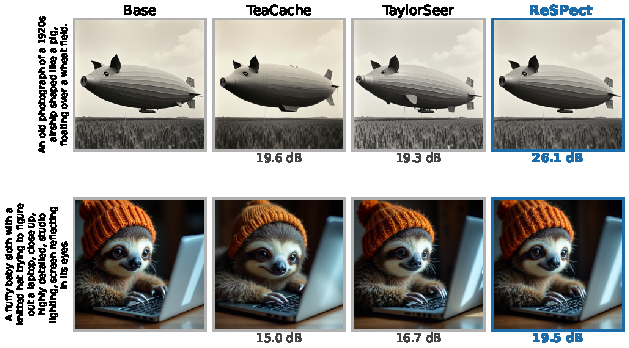
\includegraphics[width=\textwidth]{respect_flux_qual.pdf}
  \caption[ReSPect on FLUX.1-dev: qualitative comparison]{FLUX.1-dev at $\delta=0.6$. The PSNR with respect to the uncached image is printed under each panel (top prompt: 19.6 / 19.3 / 26.1\,dB; bottom prompt: 15.0 / 16.7 / 19.5\,dB for TeaCache / TaylorSeer / ReSPect). TeaCache and TaylorSeer use equal or more compute.}
  \label{fig:respect-fluxqual}
\end{figure}

\begin{figure}[t]
  \centering
  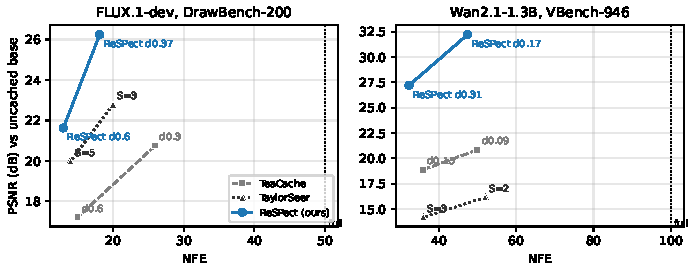
\includegraphics[width=\textwidth]{respect_psnr_nfe.pdf}
  \caption[ReSPect: PSNR versus compute]{PSNR versus compute (NFE) on FLUX.1-dev, DrawBench-200 (left) and Wan2.1-1.3B, VBench-946 (right). ReSPect is compared with published TeaCache and TaylorSeer operating points; the dotted line marks uncached compute. The Wan2.1 gain at the aggressive budget is $+8.32$\,dB.}
  \label{fig:respect-psnr}
\end{figure}

\subsection{Text-to-video results}
The gains are largest on video (\cref{tab:respect-video}). On Wan2.1, ReSPect reaches 32.21\,dB at $\delta=0.17$ ($+11.4$\,dB over TeaCache) and 27.20\,dB at $\delta=0.31$ ($+8.3$\,dB), with LPIPS less than a third of any baseline. On HunyuanVideo the margins are $+9.9$\,dB and $+8.8$\,dB at $\delta=0.27$ and $0.48$. \Cref{fig:respect-videoqual} shows opening frames and \cref{fig:respect-strip-hy,fig:respect-strip-wan} full frame strips.

\begin{table}[t]
  \centering
  \small
  \setlength{\tabcolsep}{4pt}
  \caption[ReSPect on HunyuanVideo and Wan2.1]{Text-to-video results on VBench (480p, 65 frames, 50 steps). Latencies on one NVIDIA B200 (bf16); speedup is relative to the original latency (HunyuanVideo 77.3\,s, Wan2.1 28.8\,s).}
  \label{tab:respect-video}
  \resizebox{\textwidth}{!}{%
  \begin{tabular}{@{}lcccc@{\hspace{10pt}}lcccc@{}}
    \toprule
    \multicolumn{5}{c}{HunyuanVideo (orig.\ 77.3\,s)} & \multicolumn{5}{c}{Wan2.1-1.3B (orig.\ 28.8\,s)} \\
    \cmidrule(r){1-5}\cmidrule(l){6-10}
    Method & PSNR$\uparrow$ & SSIM$\uparrow$ & LPIPS$\downarrow$ & Lat./Speedup & Method & PSNR$\uparrow$ & SSIM$\uparrow$ & LPIPS$\downarrow$ & Lat./Speedup \\
    \midrule
    Vanilla 25 & 19.97 & 0.731 & 0.263 & 38.7 / $2.00\times$ & TeaCache 0.09 & 20.84 & 0.721 & 0.171 & 14.9 / $1.93\times$ \\
    TeaCache 0.12 & 23.40 & 0.805 & 0.133 & 42.0 / $1.84\times$ & TaylorSeer S2 & 16.15 & 0.543 & 0.336 & 15.3 / $1.88\times$ \\
    TaylorSeer S2 & 24.14 & 0.820 & 0.152 & 42.0 / $1.84\times$ & \textbf{ReSPect 0.17} & \textbf{32.21} & \textbf{0.947} & \textbf{0.033} & 14.8 / $1.95\times$ \\
    \textbf{ReSPect 0.27} & \textbf{34.07} & \textbf{0.946} & \textbf{0.046} & 39.9 / $1.94\times$ & & & & & \\
    \midrule
    Vanilla 15 & 17.49 & 0.662 & 0.371 & 23.2 / $3.33\times$ & TeaCache 0.15 & 18.88 & 0.645 & 0.245 & 10.4 / $2.77\times$ \\
    TeaCache 0.2 & 20.42 & 0.734 & 0.172 & 30.2 / $2.56\times$ & TaylorSeer S3 & 14.18 & 0.453 & 0.455 & 11.2 / $2.57\times$ \\
    TaylorSeer S3 & 20.42 & 0.733 & 0.242 & 30.2 / $2.56\times$ & \textbf{ReSPect 0.31} & \textbf{27.20} & \textbf{0.888} & \textbf{0.082} & 10.9 / $2.63\times$ \\
    \textbf{ReSPect 0.48} & \textbf{29.20} & \textbf{0.891} & \textbf{0.100} & 27.9 / $2.77\times$ & & & & & \\
    \bottomrule
  \end{tabular}}
\end{table}

\begin{figure}[t]
  \centering
  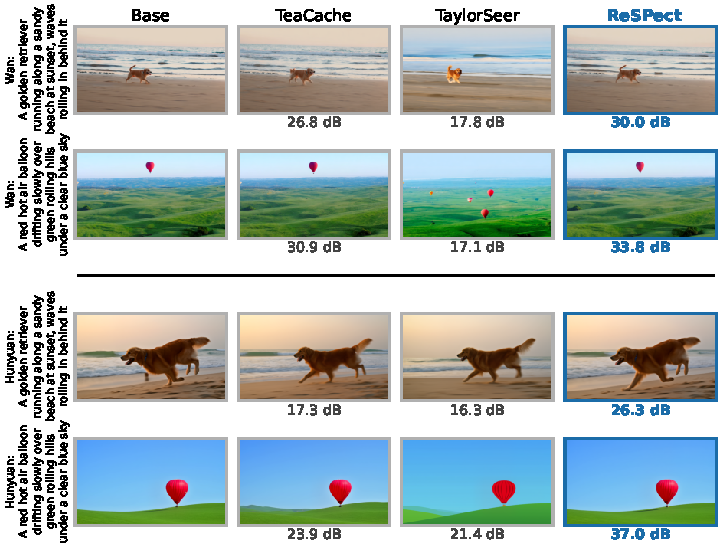
\includegraphics[width=0.92\textwidth]{respect_video_qual.pdf}
  \caption[ReSPect on video: opening frames]{Opening frames on Wan2.1 and HunyuanVideo for two prompts (a golden retriever on a beach, a hot-air balloon over hills). ReSPect uses $\delta=0.31$ (Wan2.1) and $0.48$ (HunyuanVideo) with less compute than TeaCache and TaylorSeer; the PSNR of each panel is printed below it.}
  \label{fig:respect-videoqual}
\end{figure}

\subsection{Cost of the forecaster and comparison with SeaCache}
A latency column combines the effects of schedule and reconstructor. Running copy-reuse and the forecast in one harness at the same $\delta$ fixes the schedule, because the gate reads the modulated block input and the reconstructor does not change where it fires; the realised NFE is then identical. \Cref{tab:respect-cost} shows that the forecast adds 1.7--4.3\% wall-clock time over copy-reuse. \Cref{tab:respect-seacache} compares ReSPect with SeaCache's copy-reuse at matched schedules: the forecast wins on PSNR and SSIM at every setting, by $+0.79$\,dB on FLUX $\delta=0.37$ ($n=200$), $+0.49$\,dB on FLUX $\delta=0.6$ ($n=20$) and $+0.93$\,dB on Wan2.1 $\delta=0.31$ ($n=20$), with LPIPS down 18\% where measured. We attribute this to the forecast tracking the trajectory between evaluations, whereas copy-reuse holds the last residual fixed.

\begin{table}[t]
  \centering
  \begin{minipage}[t]{0.52\textwidth}
  \centering
  \small
  \caption[Cost of the ReSPect forecaster]{Cost of the reconstructor at a fixed schedule (same gate and $\delta$, one B200). NFE is identical within each pair.}
  \label{tab:respect-cost}
  \setlength{\tabcolsep}{3pt}
  \resizebox{\linewidth}{!}{%
  \begin{tabular}{@{}lccccc@{}}
    \toprule
    Model & $\delta$ & NFE & Reuse (s) & Forecast (s) & $\Delta$ \\
    \midrule
    FLUX.1-dev & 0.3 & 21 & 2.38 & 2.47 & +3.8\% \\
    FLUX.1-dev & 0.6 & 13 & 1.55 & 1.61 & +3.9\% \\
    Wan2.1-1.3B & 0.17 & 46 & 14.31 & 14.80 & +3.4\% \\
    Wan2.1-1.3B & 0.31 & 32 & 10.49 & 10.94 & +4.3\% \\
    HunyuanVideo & 0.27 & 24 & 39.20 & 39.86 & +1.7\% \\
    HunyuanVideo & 0.48 & 16 & 27.38 & 27.90 & +1.9\% \\
    \bottomrule
  \end{tabular}}
  \end{minipage}\hfill
  \begin{minipage}[t]{0.45\textwidth}
  \centering
  \small
  \caption[ReSPect versus SeaCache at matched schedules]{ReSPect vs.\ SeaCache copy-reuse at matched schedules (same $\delta$, prompts and gate; only the reconstruction differs).}
  \label{tab:respect-seacache}
  \setlength{\tabcolsep}{3pt}
  \resizebox{\linewidth}{!}{%
  \begin{tabular}{@{}llccc@{}}
    \toprule
    Setting & Method & NFE & PSNR & SSIM \\
    \midrule
    FLUX $\delta{=}0.37$ & SeaCache & 18.1 & 25.45 & 0.880 \\
    ($n{=}200$) & ReSPect & 18.1 & 26.24 & 0.895 \\
    FLUX $\delta{=}0.6$ & SeaCache & 13.0 & 23.08 & 0.848 \\
    ($n{=}20$) & ReSPect & 13.0 & 23.57 & 0.852 \\
    Wan $\delta{=}0.31$ & SeaCache & 32.4 & 28.80 & 0.904 \\
    ($n{=}20$) & ReSPect & 32.3 & 29.73 & 0.917 \\
    \bottomrule
  \end{tabular}}
  \end{minipage}
\end{table}

\subsection{Ablations}\label{sec:respect-ablations}
\paragraph{Degree and penalty.} On FLUX.1-dev at $\delta=0.6$ (first 20 prompts, one shared base run), varying $M$ and $\lambda$ around the defaults yields a flat optimum (\cref{tab:respect-msweep}): $M\in\{4,6\}$ and $\lambda\in\{0.01,0.1\}$ agree to within 0.15\,dB.

\begin{table}[t]
  \centering
  \small
  \caption[ReSPect: sweeps of $M$ and $\lambda$]{Sweeps of the Chebyshev degree $M$ ($\lambda=0.1$) and the ridge penalty $\lambda$ ($M=4$) on FLUX.1-dev, $\delta=0.6$, $n=20$. The default is the first row of each block.}
  \label{tab:respect-msweep}
  \begin{tabular}{@{}lcc@{\hspace{24pt}}lcc@{}}
    \toprule
    Setting & PSNR$\uparrow$ & SSIM$\uparrow$ & Setting & PSNR$\uparrow$ & SSIM$\uparrow$ \\
    \midrule
    Default ($M=4$) & 23.57 & 0.852 & Default ($\lambda=0.1$) & 23.57 & 0.852 \\
    $M=2$ & 23.02 & 0.845 & $\lambda=0.01$ & 23.56 & 0.853 \\
    $M=6$ & 23.72 & 0.855 & $\lambda=1.0$ & 23.38 & 0.847 \\
    \bottomrule
  \end{tabular}
\end{table}

\paragraph{Reconstructor ablations against copy-reuse.} All arms of \cref{fig:respect-ablation} share one base run, so every $\Delta$dB is paired against the same copy-reuse baseline, at the aggressive budgets (FLUX $\delta=0.6$, Wan $\delta=0.31$) on fixed 20-prompt subsets.
\begin{itemize}
  \item \emph{Blend weight $w$.} Pure Taylor ($w=0$) is strong wherever neighbouring evaluations carry the signal: $+2.30$\,dB on Wan2.1 and $+0.50$\,dB on FLUX. Pure Chebyshev ($w=1$) fails precisely where the fit is least determined: $-1.68$\,dB on Wan2.1, with its long skip runs, and $+0.09$\,dB (about copy-reuse) on FLUX. The fixed $w=0.5$ remains at or above copy-reuse on either model ($+0.49$/$+0.93$\,dB): a robust compromise rather than a per-subset optimum.
  \item \emph{Warm-up threshold.} Blending before the fit is determined lets the penalty dominate the data. A warm-up of 8 attains the largest FLUX gain ($+0.68$\,dB) but lies within noise of the default; longer Taylor-only spans (12--24) never accumulate enough observations to blend at this budget and coincide with pure Taylor ($+0.50$\,dB).
  \item \emph{Window $K$.} $K=32$ matches $K=100$ to three decimals ($+0.491$ vs.\ $+0.491$\,dB): per-prompt buffers rarely exceed about 40 observations, so the $\sigma_{\min}$ gains of \cref{lem:respect-ridge} saturate early and $K=100$ is a conservative default.
  \item \emph{Gate reference.} Refreshing the gate reference at every step rather than only at evaluated steps contributes $+2.50$\,dB on HunyuanVideo at matched compute.
\end{itemize}

\begin{figure}[t]
  \centering
  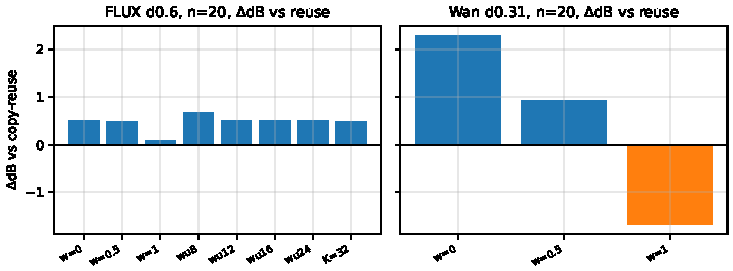
\includegraphics[width=0.95\textwidth]{respect_ablation.pdf}
  \caption[ReSPect: reconstructor ablations]{Reconstructor ablations ($\Delta$dB against copy-reuse, paired on one shared base run per panel). Left: FLUX.1-dev, $\delta=0.6$, $n=20$ (blend weights, warm-ups ``wu'' of 8--24, window $K=32$). Right: Wan2.1, $\delta=0.31$, $n=20$. Pure Taylor dominates on Wan2.1 while the blend remains at or above copy-reuse; pure Chebyshev fails on long skip runs.}
  \label{fig:respect-ablation}
\end{figure}

\paragraph{Where compute is spent.} Refresh histograms concentrate compute early along the trajectory, in accordance with the spectral prior: evaluations are dense while $G_t$ is narrow (content forming) and sparse as the passband widens. Skip rates concentrate tightly per budget (\cref{fig:respect-skiprate}), and PSNR-versus-refresh curves follow the full-compute reference monotonically at both $\delta$ settings, with the gap to copy-reuse widening at lower refresh ratios, exactly where the reuse bound \cref{eq:respect-reuse} loosens while the uniform bound \cref{eq:respect-trunc} remains tight. \Cref{fig:respect-perprompt} shows per-prompt SSIM and LPIPS.

\begin{figure}[t]
  \centering
  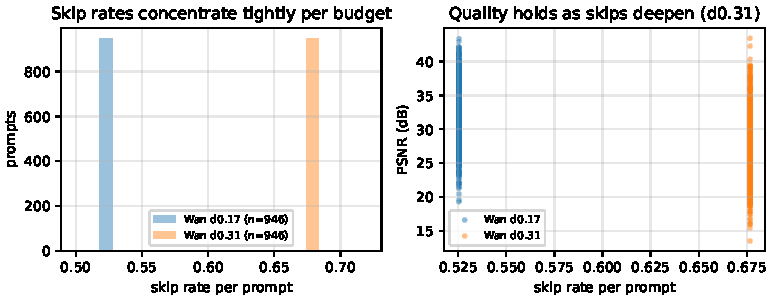
\includegraphics[width=0.95\textwidth]{respect_skiprate.pdf}
  \caption[ReSPect: skip rates per prompt]{Compute concentrates early and quality tracks full compute (Wan2.1, VBench-946). Left: per-prompt skip-rate histograms at $\delta=0.17$ and $0.31$. Right: per-prompt PSNR versus skip rate.}
  \label{fig:respect-skiprate}
\end{figure}

\begin{figure}[t]
  \centering
  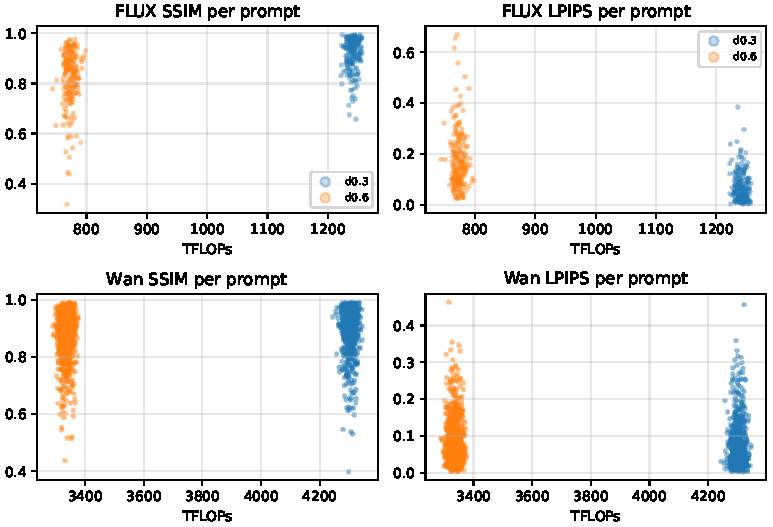
\includegraphics[width=0.85\textwidth]{respect_perprompt.pdf}
  \caption[ReSPect: per-prompt SSIM and LPIPS]{Per-prompt SSIM and LPIPS at each configuration's TFLOPs. Top: FLUX.1-dev, DrawBench-200. Bottom: Wan2.1, VBench-946.}
  \label{fig:respect-perprompt}
\end{figure}

\subsection{Qualitative clips}
\Cref{tab:respect-clips} gives frame-averaged metrics for two clips per video model, generated in our harness at $\delta=0.31$ (Wan2.1, 32 forward passes) and $\delta=0.48$ (HunyuanVideo, 16); TeaCache and TaylorSeer run at their published operating points and use more compute. ReSPect uses the least compute and leads on every clip and metric. On the HunyuanVideo balloon clip, TaylorSeer renders a different scene entirely and retains it for the whole clip; on Wan2.1 it hallucinates three additional balloons (\cref{fig:respect-strip-hy,fig:respect-strip-wan}). The retriever prompt is a difficult motion case in which all caches degrade while the ordering is preserved.

\begin{table}[t]
  \centering
  \small
  \caption[ReSPect: per-clip comparison]{Per-clip comparison: frame-averaged PSNR, SSIM and LPIPS against the uncached same-seed reference over all 65 frames. NFE is forward passes per clip (Wan2.1 base 100, HunyuanVideo base 50).}
  \label{tab:respect-clips}
  \begin{tabular}{@{}llcccc@{}}
    \toprule
    Clip & Method & PSNR$\uparrow$ & SSIM$\uparrow$ & LPIPS$\downarrow$ & NFE \\
    \midrule
    \multirow{3}{*}{Wan retriever} & TeaCache & 27.07 & 0.892 & 0.109 & 38 \\
     & TaylorSeer & 17.91 & 0.656 & 0.384 & 36 \\
     & ReSPect & \textbf{30.96} & \textbf{0.937} & \textbf{0.066} & 32 \\
    \midrule
    \multirow{3}{*}{Wan balloon} & TeaCache & 31.29 & 0.918 & 0.064 & 38 \\
     & TaylorSeer & 17.60 & 0.568 & 0.321 & 36 \\
     & ReSPect & \textbf{34.87} & \textbf{0.950} & \textbf{0.031} & 32 \\
    \midrule
    \multirow{3}{*}{Hunyuan retriever} & TeaCache & 16.32 & 0.669 & 0.322 & 18 \\
     & TaylorSeer & 15.24 & 0.643 & 0.379 & 18 \\
     & ReSPect & \textbf{26.04} & \textbf{0.878} & \textbf{0.089} & 16 \\
    \midrule
    \multirow{3}{*}{Hunyuan balloon} & TeaCache & 25.80 & 0.914 & 0.046 & 18 \\
     & TaylorSeer & 21.52 & 0.903 & 0.117 & 18 \\
     & ReSPect & \textbf{37.41} & \textbf{0.980} & \textbf{0.005} & 16 \\
    \bottomrule
  \end{tabular}
\end{table}

\begin{figure}[p]
  \centering
  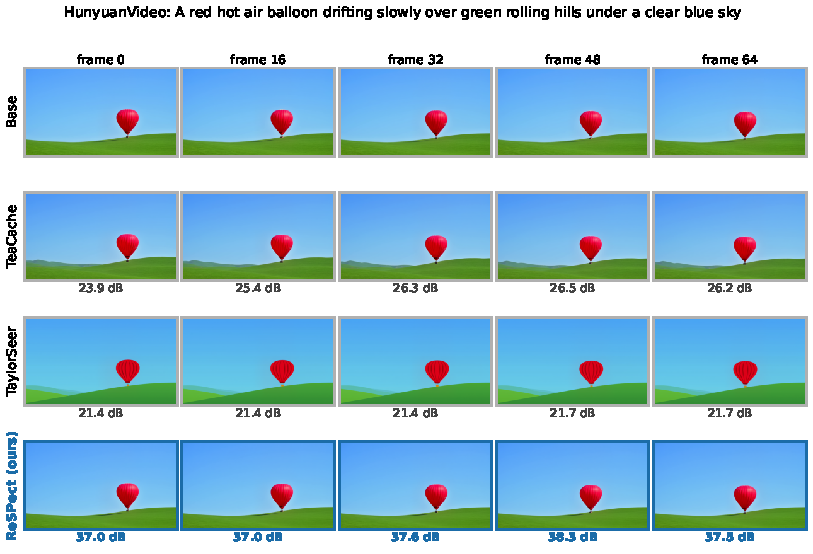
\includegraphics[width=\textwidth]{respect_strip_hunyuan.pdf}
  \caption[ReSPect: HunyuanVideo frame strip]{HunyuanVideo, balloon clip, $\delta=0.48$ (16 NFE), frames 0, 16, 32, 48 and 64. Averaged over all 65 frames, ReSPect scores 37.41\,dB against 25.80\,dB (TeaCache) and 21.52\,dB (TaylorSeer).}
  \label{fig:respect-strip-hy}
  \vspace{0.6cm}
  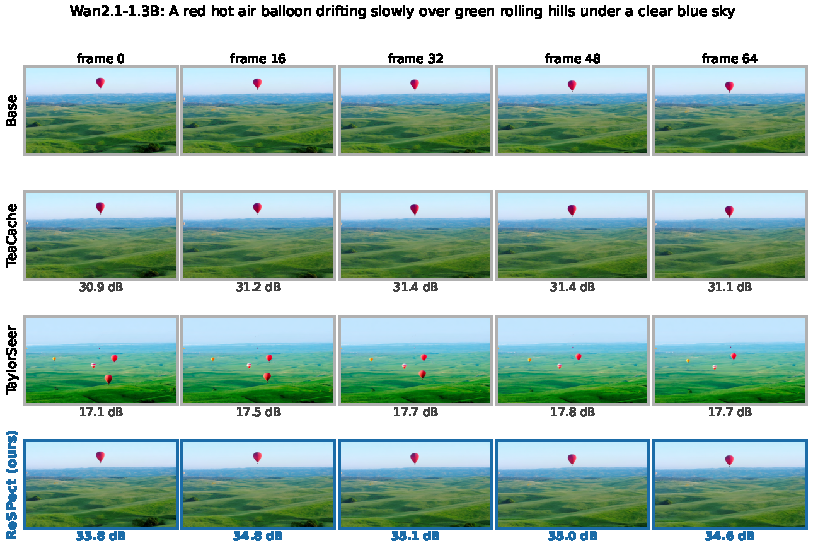
\includegraphics[width=\textwidth]{respect_strip_wan.pdf}
  \caption[ReSPect: Wan2.1 frame strip]{Wan2.1-1.3B, balloon clip, $\delta=0.31$ (32 NFE). TaylorSeer hallucinates three additional balloons and retains them for the whole clip.}
  \label{fig:respect-strip-wan}
\end{figure}

%% ------------------------------------------------------------------------------------------------
\section{Discussion and limitations}\label{sec:respect-discussion}

ReSPect couples a linear-MMSE-motivated gate with residual-space forecasting. At matched or lower compute it improves over the strongest compared baseline by up to 11.4\,dB on Wan2.1, 9.9\,dB on HunyuanVideo and 3.46\,dB on FLUX.1-dev, with the largest gains under long skips, particularly for video. Its limitations are the following.
\begin{itemize}
  \item Gains are largest when many steps are skipped; under rapid content drift the gate evaluates densely and little residual error remains for any predictor to reduce.
  \item The blend weight is fixed at $w=0.5$ rather than scheduled.
  \item Content-aware gates need not realise equal skip rates at a shared $\delta$, so comparisons must be made at matched compute.
  \item Most importantly for the next chapter, ReSPect is still an \emph{open-loop} predictor: when the next computed step reveals the forecast error of a skipped run, that error has already been integrated into the latent, and ReSPect uses the new observation only to predict the \emph{next} run. The forecast improves the upcoming steps but never revisits the past ones.
\end{itemize}
The last point led to KalSea, which replaces the regression by a state-space model whose smoother can correct the past gap (\cref{ch:kalsea}).
